% Preámbulo modular para presentaciones Beamer (Modelación Estadística)
% Diseño y paleta institucional del Tecnológico de Monterrey

\documentclass[aspectratio=169,xcolor={dvipsnames,table}]{beamer}

\usepackage[utf8]{inputenc}
\usepackage[spanish,mexico]{babel}
\usepackage{amsmath,amssymb,amsfonts,mathtools}
\usepackage{graphicx}
\usepackage{listings}
\usepackage{booktabs}
\usepackage{tikz}
\usetikzlibrary{matrix,arrows,decorations.pathmorphing,shapes.geometric,positioning}

% Paleta Institucional Tecnológico de Monterrey
\definecolor{TecAzul}{HTML}{0039A6}       % Azul TEC: color primario institucional
\definecolor{TecAzulOscuro}{HTML}{1A2E51} % Azul marino oscuro
\definecolor{TecRojo}{HTML}{EC2661}       % Rojo de acento (paleta miTec)
\definecolor{TecGris}{HTML}{646464}       % Gris neutro para comentarios y subtítulos
\definecolor{TecFondoBloque}{HTML}{F4F6F9}% Fondo suave para bloques

% Configuración de Tema Beamer
\usetheme{Boadilla}
\usecolortheme[named=TecAzulOscuro]{structure}
\setbeamercolor{alerted text}{fg=TecRojo}
\setbeamercolor{palette primary}{bg=TecAzulOscuro,fg=white}
\setbeamercolor{palette secondary}{bg=TecAzul,fg=white}
\setbeamercolor{palette tertiary}{bg=TecAzulOscuro!80!black,fg=white}
\setbeamercolor{title}{fg=TecAzulOscuro,bg=TecFondoBloque}
\setbeamercolor{frametitle}{fg=TecAzulOscuro,bg=TecFondoBloque}

% Bloques personalizados elegantes
\setbeamercolor{block title}{bg=TecAzulOscuro,fg=white}
\setbeamercolor{block body}{bg=TecFondoBloque,fg=black}
\setbeamercolor{block title alerted}{bg=TecRojo,fg=white}
\setbeamercolor{block body alerted}{bg=TecRojo!8,fg=black}
\setbeamercolor{block title example}{bg=TecAzul,fg=white}
\setbeamercolor{block body example}{bg=TecAzul!8,fg=black}

% Redondear bordes y añadir sombra sutil
\setbeamertemplate{blocks}[rounded][shadow=true]
\setbeamertemplate{navigation symbols}{}

% Pie de página limpio con número de diapositiva
\setbeamertemplate{footline}{
  \leavevmode%
  \hbox{%
  \begin{beamercolorbox}[wd=.7\paperwidth,ht=2.25ex,dp=1ex,left]{author in head/foot}%
    \hspace*{2ex}\insertshortauthor~~(\insertshortinstitute) \hfill \insertshorttitle
  \end{beamercolorbox}%
  \begin{beamercolorbox}[wd=.3\paperwidth,ht=2.25ex,dp=1ex,right]{date in head/foot}%
    \insertshortdate{}\hspace*{2em}
    \insertframenumber{} / \inserttotalframenumber\hspace*{2ex}
  \end{beamercolorbox}}%
  \vskip0pt%
}

% Configuración de Listings de Python para visualización pedagógica de código
\lstset{
    language=Python,
    basicstyle=\ttfamily\footnotesize,
    keywordstyle=\color{TecAzulOscuro}\bfseries,
    stringstyle=\color{TecRojo},
    commentstyle=\color{TecGris}\itshape,
    showstringspaces=false,
    breaklines=true,
    frame=lines,
    rulecolor=\color{TecAzulOscuro!30},
    backgroundcolor=\color{TecFondoBloque},
    aboveskip=0.5em,
    belowskip=0.5em,
    literate={á}{{\'a}}1 {é}{{\'e}}1 {í}{{\'i}}1 {ó}{{\'o}}1 {ú}{{\'u}}1
             {Á}{{\'A}}1 {É}{{\'E}}1 {Í}{{\'I}}1 {Ó}{{\'O}}1 {Ú}{{\'U}}1
             {ñ}{{\~n}}1 {Ñ}{{\~N}}1 {¿}{{?`}}1 {¡}{{!`}}1
}

% Metadatos institucionales por defecto
\title[Modelación Estadística]{Modelación Estadística para Ciencia de Datos e Ingeniería}
\author[J. Castillo Colmenares]{Juliho David Castillo Colmenares}
\institute[Tec de Monterrey]{Tecnológico de Monterrey \\ Escuela de Ingeniería y Ciencias}
\date{\today}


\title{Medidas de Tendencia Central}
\subtitle{Sección 1.2 — Modelación Estadística para Ciencia de Datos}
\author[J. Castillo Colmenares]{Juliho Castillo Colmenares}
\institute{Tecnológico de Monterrey}
\date{}

\begin{document}

% Slide 1: Portada
\begin{frame}[plain]
  \titlepage
\end{frame}

% Slide 2: Hoja de Ruta del Capítulo e Indicador de Posición
\begin{frame}{Hoja de Ruta — Capítulo 01: Estadística Descriptiva}
  ¿Dónde estamos en nuestro recorrido por la estadística básica? \pause
  \begin{itemize}
    \item \textbf{01.01 Introducción a la estadística descriptiva} \emph{(Completado)} \pause
    \item \color{TecRojo}\textbf{01.02 Medidas de tendencia central \emph{(Hoy)}}\color{black} \pause
    \item \textbf{01.03 Medidas de dispersión} \emph{(Siguiente sesión)}
  \end{itemize}
  \vspace{1em}
  \begin{block}{Objetivo de la Sección 1.2}
    Comprender y calcular el centro de un conjunto de datos matemáticamente (media y pivote) y de forma robusta frente a ruido extremo (mediana y moda).
  \end{block}
\end{frame}

% Slide 3: Reto Rápido en Equipo (Trigger Question)
\begin{frame}{Reto Rápido en Equipo}
  \begin{alertblock}{Situación en el Entorno Laboral (Pregunta Gatillo)}
    En una pequeña empresa de inteligencia artificial, cuatro programadores ganan $\$30,000$ pesos al mes cada uno. Hoy se contrata a un nuevo director ejecutivo con un sueldo mensual de $\$380,000$ pesos.
    \vspace{0.6em}
    \begin{enumerate}
      \item ¿Cuál es el sueldo promedio de los 5 integrantes de la empresa? \pause
      \item Si el departamento de recursos humanos reporta ese promedio en sus vacantes, ¿está diciendo la verdad sobre lo que gana un empleado típico? \pause
      \item ¿Qué otra medida descriptiva reflejaría con mayor honestidad la realidad salarial de la oficina?
    \end{enumerate}
  \end{alertblock}
\end{frame}

% Slide 4A: Conclusiones de la Reflexión en el Aula (Análisis)
\begin{frame}{Conclusiones de la Reflexión en el Aula — Análisis}
  \begin{itemize}
    \item \textbf{El Promedio Numérico:} El cálculo arroja $\frac{4(30,000) + 380,000}{5} = \$100,000$ pesos mensuales. \pause
    \item \textbf{Distorsión por Valores Atípicos:} Ningún programador gana $\$100,000$. El salario del director empuja la media drásticamente hacia arriba, creando un espejismo estadístico. \pause
    \item \textbf{El Valor de la Mediana:} Al ordenar los sueldos ($30, 30, \mathbf{30}, 30, 380$), el valor central ($\$30,000$) representa la auténtica experiencia del trabajador. \pause
    \item \textbf{Lección Clave:} En Ciencia de Datos, la media no es suficiente; debemos saber cuándo emplear medidas robustas.
  \end{itemize}
\end{frame}

% Slide 4B: Conclusiones de la Reflexión en el Aula (Respuestas)
\begin{frame}{Conclusiones de la Reflexión en el Aula — Respuestas}
  \begin{block}{Respuestas Formales al Reto Rápido en Equipo}
    \begin{enumerate}
      \item \textbf{Promedio aritmético:} $\$100,000$ pesos mensuales. \pause
      \item \textbf{¿Es representativo?} No refleja al empleado típico; el $80\%$ del personal gana menos de una tercera parte de esa cifra. \pause
      \item \textbf{Medida honesta:} La \textbf{Mediana ($\tilde{X}$)} o la \textbf{Moda ($M_o$)}, ya que son inmunes a la distorsión del ejecutivo estrella.
    \end{enumerate}
  \end{block}
\end{frame}

% Slide 5: La Media Aritmética y su Propiedad Fundamental
\begin{frame}{La Media Aritmética ($\bar{X}$)}
  La \textbf{media aritmética} es el promedio estándar de un conjunto de $N$ observaciones $X_1, X_2, \dots, X_N$:
  \begin{align}
    \bar{X} = \dfrac{1}{N} \sum_{i=1}^{N} X_i
  \end{align}
  \pause
  \begin{block}{Propiedad del Centro de Gravedad}
    La suma algebraica de las desviaciones de todos los datos respecto a su media aritmética es exactamente igual a cero:
    \begin{align}
      \sum_{i=1}^{N} (X_i - \bar{X}) = 0
    \end{align}
    Esto demuestra que $\bar{X}$ actúa como el punto de equilibrio físico (centro de masa) de la distribución.
  \end{block}
\end{frame}

% Slide 6: El Concepto de Pivote (P)
\begin{frame}{El Concepto de Pivote ($P$)}
  Cuando los datos tienen valores numéricos grandes o cercanos entre sí, podemos simplificar las operaciones aritméticas utilizando un valor arbitrario de referencia llamado \textbf{Pivote ($P$)}. \pause
  \begin{itemize}
    \item Sea $d_i = X_i - P$ la desviación de cada dato respecto al pivote $P$. \pause
    \item Demostraremos que la media real puede reconstruirse sumando al pivote el promedio de esas desviaciones:
  \end{itemize}
  \begin{align}
    \bar{X} = P + \dfrac{1}{N} \sum_{i=1}^{N} d_i
  \end{align}
  \pause
  \begin{block}{Ventaja Algorítmica}
    Esta fórmula previene el desbordamiento flotante (\emph{floating-point overflow}) al sumar millones de números grandes en computación, siendo la base de los algoritmos de media iterativa en Big Data.
  \end{block}
\end{frame}

% Slide 7: La Mediana y la Moda
\begin{frame}{Medidas Robustas: Mediana y Moda}
  \begin{itemize}
    \item \textbf{La Mediana ($\tilde{X}$):} Es el valor que divide a la muestra ordenada en dos mitades exactas ($50\%$ inferior y $50\%$ superior).
      \begin{itemize}
        \item Si $N$ es impar, es el dato en la posición central.
        \item Si $N$ es par, es el promedio de los dos datos centrales.
      \end{itemize}
    \pause
    \item \textbf{La Moda ($M_o$):} Es el valor que se repite con mayor frecuencia en el conjunto de observaciones. Puede no existir o haber múltiples modas (bimodal, multimodal). \pause
  \end{itemize}
  \vspace{0.4em}
  \begin{block}{Punto de Quiebre (\emph{Breakdown Point})}
    La mediana tiene un punto de quiebre del $50\%$: puede resistir que hasta la mitad de los datos sean errores corruptos o extremos sin corromperse infinitamente. La media tiene un punto de quiebre de $0\%$.
  \end{block}
\end{frame}

% Slide 8: Tendencia Central en Datos Agrupados
\begin{frame}{Tendencia Central en Datos Agrupados}
  Cuando procesamos tablas de frecuencias con $K$ clases o intervalos de frecuencias relativas/absolutas: \pause
  \begin{itemize}
    \item Sea $f_i$ la frecuencia absoluta de la clase $i$ y sea $X_i$ la \textbf{marca de clase} (el punto medio del intervalo). \pause
    \item La media aproximada para datos agrupados se pondera por su frecuencia:
  \end{itemize}
  \begin{align}
    \bar{X}_{\text{agrupada}} = \dfrac{\sum_{i=1}^{K} f_i X_i}{\sum_{i=1}^{K} f_i} = \dfrac{1}{n} \sum_{i=1}^{K} f_i X_i
  \end{align}
  \pause
  \begin{alertblock}{Nota Práctica}
    El cálculo agrupado es una aproximación muy precisa al cálculo crudo, ideal cuando solo conservamos histogramas agregados por restricciones de privacidad o almacenamiento.
  \end{alertblock}
\end{frame}

% Slide 9A: Laboratorio de Python En Vivo (Medidas Clásicas)
\begin{frame}{Laboratorio en Python: Medidas Clásicas}
  Cálculo exploratorio de Media Aritmética, Mediana y Moda usando NumPy y SciPy.
  \\ Script: \texttt{\footnotesize presentaciones/code/01\_estadistica\_descriptiva/01.02\_mean\_median\_mode.py}
  
  \vspace{0.4em}
  {\lstset{basicstyle=\ttfamily\tiny, aboveskip=0.2em, belowskip=0.2em}
  \lstinputlisting[firstline=1,lastline=16]{../../code/01_estadistica_descriptiva/01.02_mean_median_mode.py}
  }

  \vspace{0.2em}
  \begin{alertblock}{Conclusión y Verificación en Python}
    En distribuciones asimétricas (como los salarios), la mediana es el estimador más robusto del centro. La media se desplaza hacia los valores extremos y distorsiona la realidad de la mayoría.
  \end{alertblock}
\end{frame}

% Slide 14: Verificación Empírica en Python (Parte 2: Simulación y Resultados)
\begin{frame}[fragile]{Verificación Empírica en Python (2/2)}
  \footnotesize
  Ejecutamos el cálculo de métricas e imprimimos el reporte estándar (\texttt{01.02\_mean\_median\_mode.py}):

  \vspace{0.2em}
  {\lstset{basicstyle=\ttfamily\tiny, aboveskip=0.2em, belowskip=0.2em}
  \lstinputlisting[firstline=18,lastline=27]{../../code/01_estadistica_descriptiva/01.02_mean_median_mode.py}
  }

  \vspace{0.2em}
  \begin{block}{\footnotesize Salida Verificada (Consola)}
    {\fontsize{6.5pt}{7.5pt}\selectfont
    \texttt{--- Medidas Clásicas ---} \\
    \texttt{Media aritmética: 9.38 | Mediana: 9.50 | Moda: 5} \\
    \texttt{--- Cálculo con Pivote (P = 9) ---} \\
    \texttt{Desviaciones (d\_i): [-4 -1  2  0  3 -3  5  1] => Suma: 3} \\
    \texttt{Media vía pivote:   9 + (3/8) = 9.38}
    }
  \end{block}
\end{frame}

% Slide 10: Ejercicios del Libro - Nivel 1
\begin{frame}{Ejercicios del Curso — Nivel 1: Fundamental}
  \begin{block}{Problema 1.2.1 (Sencillo / Directo)}
    Escribir los términos de cada una de las siguientes sumas:
    \begin{enumerate}
      \item $\displaystyle\sum_{j=0}^{6}X_{j}=$ 
      \item $\displaystyle\sum_{k=1}^{4}\left( Y_{k}-3 \right)^{2}=$ 
      \item $\displaystyle\sum_{k=1}^{N}a=$ 
      \item $\displaystyle\sum_{n=2}^{5}{f_{n}}X_{n}= $ 
      \item $\displaystyle\sum_{m=0}^{3}\left( X_{m}-a \right)=$
    \end{enumerate}
  \end{block}
\end{frame}

% Slide 11: Ejercicios del Libro - Nivel 2
\begin{frame}{Ejercicios del Curso — Nivel 2: Operativo}
  \begin{block}{Problema 1.2.8 (Intermedio / De Desarrollo)}
    Halle la media aritmética de los números 5, 8, 11, 9, 12, 6, 14 y 10 eligiendo como \emph{pivote}:
    \begin{enumerate}
      \item $P=9$
      \item $P=20$
    \end{enumerate}
    \vspace{0.5em}
    Verifique que en ambos casos el resultado coincide exactamente con la media aritmética calculada de manera directa ($\bar{X} = 9.375$).
  \end{block}
\end{frame}

% Slide 12: Ejercicios del Libro - Nivel 3
\begin{frame}{Ejercicios del Curso — Nivel 3: Analítico}
  \begin{block}{Problema 1.2.5 (Avanzado / De Conexión)}
    Si las desviaciones de $N$ números $X_{1}, X_{2}, \dots, X_{N}$ respecto a un \emph{pivote} $P$ están dadas por $d_{i} = X_{i} - P, \; i = 1, \dots, N$ respectivamente, demostrar algebraicamente que:
    \begin{align}
      \bar{X} = P + \dfrac{\sum_{i=1}^{N} d_{i}}{N}.
    \end{align}
  \end{block}
\end{frame}

% Slide 13: Ejercicios del Libro - Nivel 4
\begin{frame}{Ejercicios del Curso — Nivel 4: Desafiante}
  \begin{columns}[c]
    \begin{column}{0.48\textwidth}
      \begin{block}{Problema 1.2.9 (Experto)}
        Utilice la marca de la clase media como pivote para calcular la estatura media de los estudiantes reportados en la tabla \ref{tab:1.2.1}. Verifique que el resultado coincide exactamente con el cálculo directo.
      \end{block}
    \end{column}
    \begin{column}{0.48\textwidth}
      \begin{figure}[ht]
        \centering
        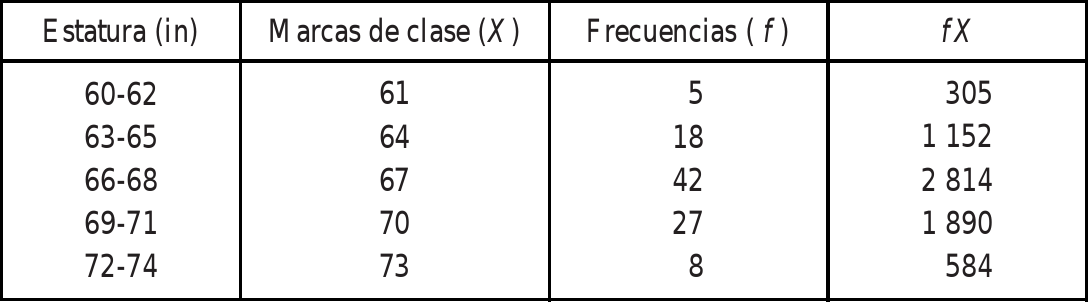
\includegraphics[width=5.8cm,keepaspectratio=true]{../../../latex/images/tab0301.png}
        \caption{Distribución de estaturas}
        \label{tab:1.2.1}
      \end{figure}
    \end{column}
  \end{columns}
\end{frame}

% Slide 14: Resumen de la Sección 1.2
\begin{frame}{Resumen de la Sección 1.2}
  \begin{block}{Lo que dominamos en esta sección}
    \begin{itemize}
      \item \textbf{Centro Numérico:} La media aritmética es el punto de equilibrio ($\sum(X_i - \bar{X}) = 0$), pero es vulnerable a valores extremos. \pause
      \item \textbf{Eficiencia por Pivote:} $\bar{X} = P + \frac{\sum d_i}{N}$ simplifica cálculos manuales y estabiliza algoritmos de computación numérica. \pause
      \item \textbf{Robustez Estadística:} La mediana y la moda aíslan anomalías en distribuciones sesgadas o con valores atípicos.
    \end{itemize}
  \end{block}
  \pause
  \vspace{0.8em}
  \begin{center}
    \color{TecAzulOscuro}\textbf{Pausa de Asimilación:} ¿Alguna duda sobre el cálculo con pivote o la elección entre media y mediana?
    \color{black}
  \end{center}
\end{frame}

% Slide 15: Conexión con el Siguiente Tema
\begin{frame}{Conexión con el Próximo Tema}
  \begin{alertblock}{Siguiente Sección: 01.03 Medidas de Dispersión}
    Dos conjuntos de datos pueden tener exactamente la misma media ($\bar{X} = 50$) y ser completamente diferentes ($[50, 50, 50]$ vs $[0, 50, 100]$).
    \vspace{0.6em}
    \\ En la \textbf{Sección 1.3} mediremos qué tan dispersos, variables o concentrados están nuestros datos a través de:
    \begin{itemize}
      \item La Varianza ($S^2$)
      \item La Desviación Estándar ($S$)
      \item El Coeficiente de Variación ($CV$)
    \end{itemize}
  \end{alertblock}
\end{frame}

\end{document}
